\section{Последовательные проверки на A100}

\subsection{Контроль BART против Copy}
Чтобы отделить эффект copy-head от различий оборудования и рецепта,
обе модели заново обучены на одной A100 в одинаковых условиях:
1M train, одна эпоха (3907 попыток шага), Val-20k, seed 42,
LR $2\cdot10^{-4}$, FP16, microbatch 128 и accumulation 2,
без gradient checkpointing и compile.

\begin{table}[htbp]
\centering\small\begin{tabular}{lrrrr}
\toprule
Модель & Token loss & Решено / 19886 & \pass{}, \% & Ошибки / 20k \\
\midrule
BART & 0.394293 & 10204 & 51.3125 & 368 \\
Copy & 0.393124 & 10203 & 51.3075 & 357 \\
\bottomrule
\end{tabular}

\caption{Сопоставимый контроль BART/Copy на A100. Ошибки кода считаются
по всем 20\,000 ответам; \pass{} --- по 19\,886 допустимым эталонам.}
\end{table}

BART решил на одну задачу больше: разница всего 0.0050 п.п.
Парно 9155 задач решены обеими моделями, 1049 --- только BART,
1048 --- только Copy. Заранее я решил выбирать более простой BART,
если Copy не превосходит его больше чем на 0.5 п.п.
\textbf{Вывод.} Я не увидел убедительного выигрыша от copy-head:
результаты отличались всего на одну задачу. Для следующих проверок
я оставил более простой BART.

\subsection{Повторение данных против разнообразия}
При неизменной архитектуре сравнивались два бюджета по четыре миллиона
предъявлений: исходный миллион, повторённый четыре раза, и четыре
миллиона различных исходных train-примеров. Обе модели обучались с нуля,
имели 15\,625 плановых попыток шага, одинаковые seed, batch, LR,
расписание и validation.

\begin{table}[htbp]
\centering\small\begin{tabular}{lrrr}
\toprule
Train / предъявления & Token loss & Решено / 19886 & \pass{}, \% \\
\midrule
1M $\times$ 4 & 0.267353 & 13445 & 67.6104 \\
4M различных & 0.250444 & 13657 & 68.6765 \\
\bottomrule
\end{tabular}

\caption{Сравнение числа различных train-примеров при одном бюджете
предъявлений. Протокол оценки: beam 4, LP 1.0, max 256.}
\label{tab:diversity}
\end{table}

\begin{figure}[htbp]
\centering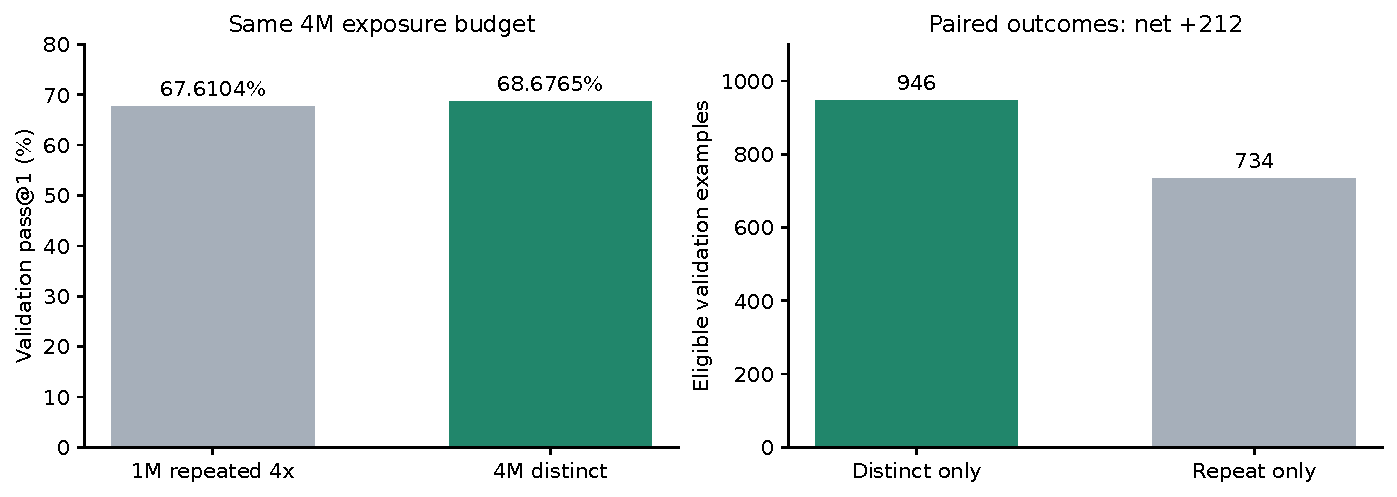
\includegraphics[width=\linewidth]{data_diversity.pdf}
\caption{Разнообразие данных: качество и парные несовпадения.
Обе модели решили 12\,711 задач; 5495 не решила ни одна.}
\end{figure}

Distinct4m решил дополнительно 212 задач (+1.0661 п.п.):
946 решены только им и 734 --- только Repeat4m.
Количество ошибок кода уменьшилось со 113 до 70 на 20\,000 ответов.
Это непосредственное основание расширить обучение на все исходные train.

Первый Repeat4m был прерван из-за взаимодействия собственного guard
с native AMP. После диагностики я продолжил его из checkpoint-14000
в отдельной папке, сохранив результаты первой попытки.
Был обработан один overflow в resumed-сессии Repeat4m
и два в Distinct4m. Поэтому равенство плановых попыток не гарантирует
равенства числа успешных обновлений. Агрегат \code{train_loss} после
resume не интерпретировался как среднее всего эксперимента.

\textbf{Вывод.} При том же бюджете предъявлений я получил более высокое
качество на различных примерах, чем при повторении одного миллиона.
Этот результат стал для меня основанием перейти к полному train.
Пока я проверил это только с одним seed и бюджетом, поэтому не переношу
наблюдение автоматически на другие объёмы и модели.

\subsection{Аудит ошибок и качества эталонов}
Выполнен ручной семантический разбор 200 случайных допустимых ошибок
Distinct4m и 200 примеров исходного train. Все 400 программ синтаксически
корректны и содержат \code{solve()}, что само по себе не подтверждает
их содержательную правильность.

В 200 train-примерах отмечены 48 несоответствий условие--код,
2 возврата неопределённой переменной, 29 проблем формулировки и 3 прочих
замечания; в 118 конкретный дефект не найден.
В выбранных 200 validation-ошибках помечены 125 сомнительных эталонов,
34 неоднозначных или неполных условия, 2 соглашения о точности;
в 39 конкретная проблема эталона не найдена.

Например, один эталон вычитает вес постороннего рюкзака из веса
постиранной одежды; два train-эталона присваивают результат одной
переменной, но возвращают неопределённую \code{result}.
Два первоначальных замечания об отсутствии \code{import math} сняты:
фактический evaluator предоставляет \code{math} в окружении.

\textbf{Вывод.} При разборе примеров с помощью Codex я увидел,
что часть ошибок метрики связана с самим корпусом и не обнаруживается
синтаксической проверкой. Я использовал эти отметки для понимания ошибок,
но не считаю их измеренной долей шума во всём датасете:
validation-примеры выбирались среди неуспехов модели.
По результатам аудита я не менял таргеты и знаменатель \pass{}
и не создавал дополнительные данные.

\subsection{Выбор beam и length penalty}
На первых 2000 строках той же Val-20k сравнены пять вариантов декодирования
Distinct4m. Допустимы 1988 эталонов; seed и checkpoint фиксированы.

\begin{table}[htbp]
\centering\small\begin{tabular}{rrrrrr}
\toprule
Beam & LP & Batch & Решено / 1988 & \pass{}, \% & A100, с \\
\midrule
2 & 1.0 & 64 & 1365 & 68.6620 & 42.55 \\
4 & 1.0 & 64 & 1378 & 69.3159 & 53.63 \\
8 & 1.0 & 32 & 1376 & 69.2153 & 95.47 \\
4 & 0.8 & 64 & 1378 & 69.3159 & 50.85 \\
4 & 1.2 & 64 & 1378 & 69.3159 & 51.74 \\
\bottomrule
\end{tabular}

\caption{Подбор декодирования на A100. Для beam 8 batch уменьшен
до 32; у остальных вариантов batch 64.}
\label{tab:decoding}
\end{table}

\begin{figure}[htbp]
\centering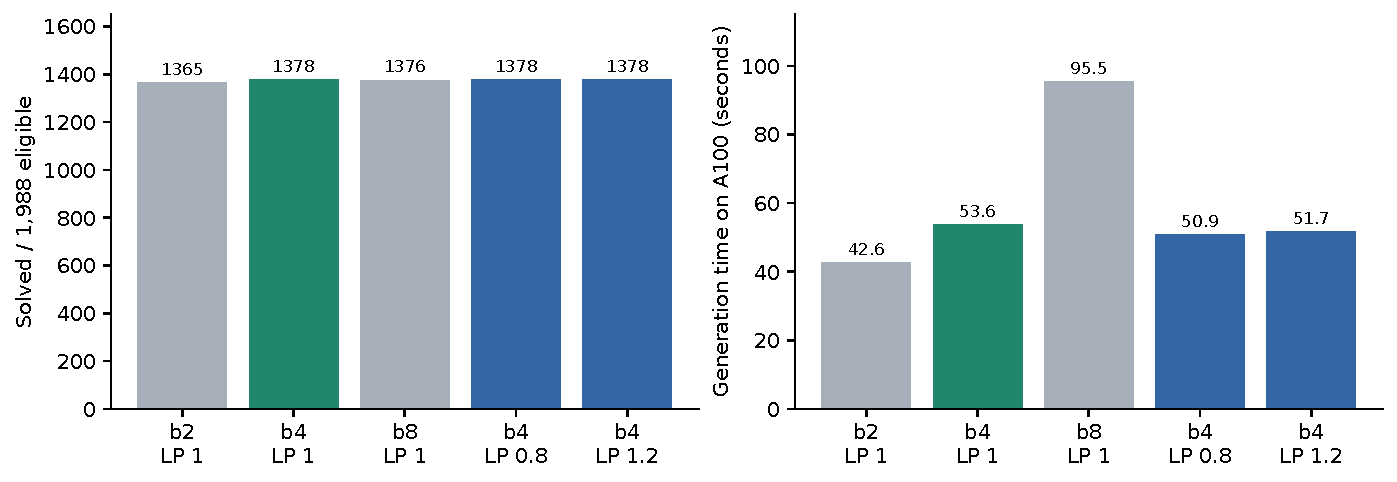
\includegraphics[width=\linewidth]{decoding.pdf}
\caption{Количество решённых задач и стоимость генерации на subset 2k.
Зелёным выделен выбранный beam 4 / LP 1.0.}
\end{figure}

По заранее заданному правилу выбирается больше решённых задач,
при равенстве --- меньший beam, затем LP ближе к 1.0.
Выбран beam 4 / LP 1.0. На полной Val-20k подтверждены
13\,657/19\,886 = 68.6765\%; все предсказания и pass-флаги совпали
с прежней оценкой Distinct4m. Генерация заняла 464.44 секунды на A100.
\textbf{Вывод.} Я оставил beam 4 / LP 1.0: увеличение beam до 8
не улучшило результат на subset, но увеличило время генерации.
От изменения LP я также не получил выигрыша по \pass{}.

\subsection{Полное обучение выбранного BART}
На основании предыдущих проверок BART 8+8/d1024/FF4096 обучен с нуля
на 11\,593\,060 train. Использованы неизменный BPE8000,
полные 118\,302 validation, FP16, seed 42, LR $2\cdot10^{-4}$,
cosine с warmup 5\%, global batch 256 = 128$\times$2,
лимиты 256/256, без compile и gradient checkpointing.
Validation и resumable checkpoint сохранялись каждые 5000 шагов.
Рецепт допускал четыре эпохи и early stopping с patience 5 по token loss.

\begin{table}[htbp]
\centering\small
\begin{tabularx}{\linewidth}{lX}
\toprule
Показатель & Результат \\
\midrule
Завершение & 23 октября, 16:26:37 МСК; exitcode 0 \\
Бюджет & 4 эпохи, 181\,144 плановых попытки шага \\
Время trial & 53\,940.95 с, около 14 ч 59 мин \\
Лучший checkpoint & 180\,000; validation token loss 0.1910213150 \\
Повторная оценка экспорта & 0.1910215739 на 7\,970\,835 целевых токенах \\
Пиковая allocated memory & 32.55 ГиБ на A100 80GB PCIe \\
Early stopping & Не сработал; достигнут предел эпох \\
AMP & 66 обработанных overflow; сохранённые loss конечны \\
\bottomrule
\end{tabularx}
\caption{Завершённое полное обучение. Повторная оценка лучших весов
не является оценкой последних обновлённых весов.}
\end{table}

\begin{figure}[htbp]
\centering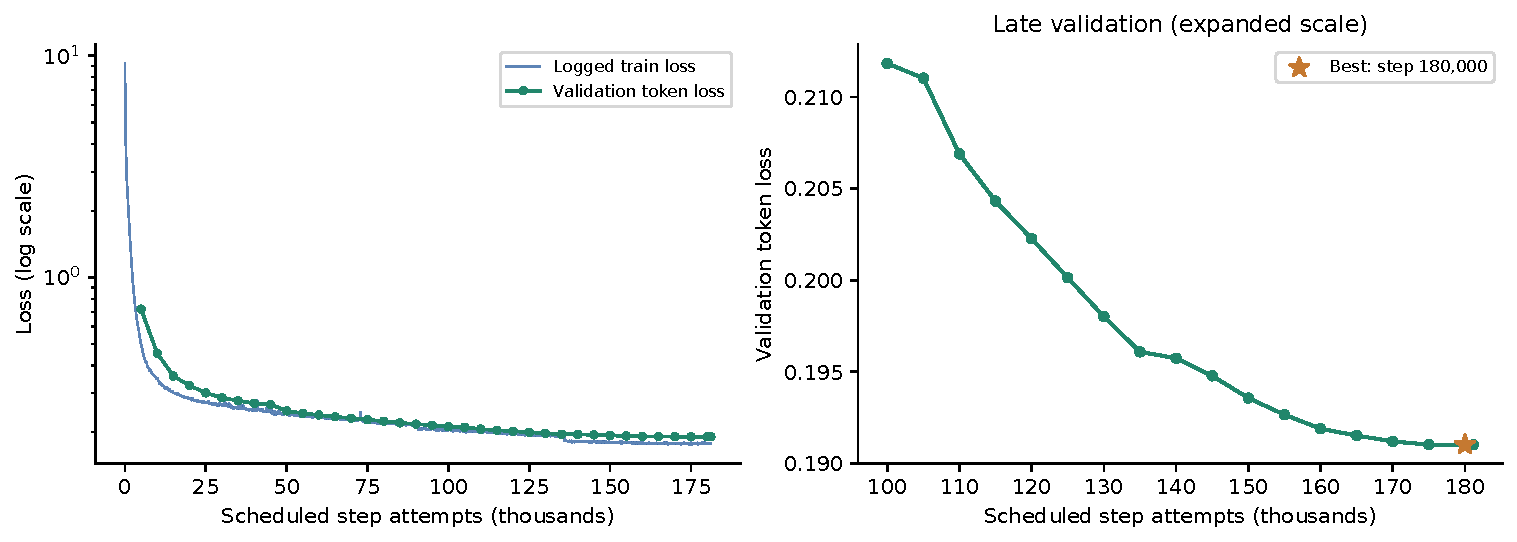
\includegraphics[width=\linewidth]{full_training.pdf}
\caption{Полное обучение BART. Слева --- обзор loss в логарифмическом
масштабе, справа --- поздняя validation с увеличенным масштабом.
Линия validation относится к весам соответствующих шагов; последняя
повторная оценка восстановленных лучших весов в неё не подставляется.}
\label{fig:full}
\end{figure}

Финальный экспорт побитово совпал с checkpoint-180000;
все 344 сохранённых тензора конечны. Лучший и последний checkpoint
с optimizer, scheduler, scaler и RNG оставлены на сервере.
Локально сохранены небольшие метрики, конфигурации и графики.

\textbf{Вывод.} Я довёл выбранную конфигурацию до четырёх эпох
и получил token loss 0.1910 на полной validation без срыва обучения.
После экспорта я отдельно проверил качество генерации и время
на официальном наборе задач на T4.

\subsection{Качество полной модели на прежней validation}
Финальный экспорт checkpoint-180000 оценён на той же Val-20k,
что Distinct4m: beam 4, LP 1.0, максимум 256 новых токенов,
один итоговый кандидат, те же 19\,886 допустимых эталонов.
Проверены идентичность всех строк и эталонных результатов, SHA256 весов,
счётчики и сохранённые pass-флаги.

\begin{table}[htbp]
\centering\small\begin{tabular}{lrrr}
\toprule
Модель / бюджет & Решено / 19886 & \pass{}, \% & Ошибки / 20k \\
\midrule
Distinct4m / 4M & 13657 & 68.6765 & 70 \\
Полный train / 4 эпохи & 14775 & 74.2985 & 32 \\
\bottomrule
\end{tabular}

\caption{Короткий Distinct4m и полностью обученный BART на одной
Val-20k. Бюджеты обучения различаются; это сравнение итоговых
конфигураций, а не опыт с одинаковым числом предъявлений.}
\label{tab:fullquality}
\end{table}

Полная модель решила дополнительно 1118 задач (+5.6220 п.п.).
Парно 13\,101 задача решена обеими моделями, 1674 --- только полной,
556 --- только Distinct4m, 4555 не решила ни одна.
Доля ошибок кода снизилась с 0.35\% до 0.16\% от всех 20\,000 ответов;
лимит длины достигнут в 9 случаях вместо 15.
Генерация полной выборки на A100 заняла 466.75 секунды,
исполнение --- 245.29 секунды.

\textbf{Вывод.} По сравнению с коротким Distinct4m я получил более высокое
качество на неизменной validation. Эту выборку я использовал
для мониторинга loss и выбора checkpoint, поэтому отдельно проверил
новую модель в официальном checker. Public 76.56\% старой модели 002
я не сравниваю напрямую с validation 74.2985\% новой модели.

\subsection{Фактический финалист на одной T4}
В приватном Colab-сеансе выполнен полный прогон официальных 1919
условий на одной Tesla T4. SHA256 весов совпал с экспортом лучшего
checkpoint-180000; порядок всех вопросов закреплён отдельно.
Использованы FP16, beam 4, LP 1.0, KV-cache, группировка по длине,
batch 128 и максимум 256 новых токенов. Входные вопросы не обрезались,
исполнение сгенерированного кода в замер не входило.

\begin{table}[htbp]
\centering\small
\begin{tabularx}{\linewidth}{lX}
\toprule
Показатель & Результат \\
\midrule
GPU / число устройств & Tesla T4 / 1 \\
Модель & Лучший BART 8+8/d1024, checkpoint-180000 \\
Официальные условия & 1919, без открытых эталонных ответов \\
Декодирование & FP16, beam 4, LP 1.0, batch 128, max 256 \\
Время инференса & 165.07 с внутри pipeline; 165.11 с внешний wall time \\
Загрузка весов, отдельно & 4.30 с \\
Пик allocated memory & 8.07 ГиБ \\
Пустые ответы / достижение лимита & 0 / 0; все ответы завершены EOS \\
Окружение & PyTorch 2.11.0+cu130, Transformers 5.10.2 \\
\bottomrule
\end{tabularx}
\caption{Измеренный протокол официальной генерации фактическим
финалистом на одной T4.}
\end{table}

Таймер включает токенизацию, сортировку по длине, переносы, генерацию,
декодирование и сборку ответов. Загрузка checkpoint, установка зависимостей
и запись файлов исключены; отдельного generation warmup не было.
Внешнее wall time также меньше 180 секунд, запас --- около 14.9 секунды.
Этот результат подтверждает выполнение ограничения в измеренном runtime;
скорость может отличаться между Colab-сеансами.

Я отправил боту файл из 1919 ответов. Результат и сравнение
с моей предыдущей посылкой приведены далее.

\subsection{Public: сравнение с прежней полной моделью 002}
\begin{table}[htbp]
\centering\small\begin{tabular}{>{\raggedright\arraybackslash}p{.30\linewidth}>{\raggedright\arraybackslash}p{.28\linewidth}>{\raggedright\arraybackslash}p{.28\linewidth}}
\toprule
Параметр & Прежняя 002 & Новая полная \\
\midrule
Encoder + decoder & 8+8 & 8+8 \\
Hidden / FFN & 768 / 3072 & 1024 / 4096 \\
Параметры, млн & 139.25 & 244.39 \\
Train / эпохи & 11\,593\,060 / 4 & 11\,593\,060 / 4 \\
BPE / seed & 8000 / 42 & 8000 / 42 \\
Global batch & 128 & 256 \\
LR & $3\cdot10^{-4}$; после 50k $10^{-4}$ & $2\cdot10^{-4}$ \\
Точность обучения & BF16 & FP16 \\
Лучший checkpoint & 360000 & 180000 \\
Token loss Val-full & 0.1927033 & 0.1910213 \\
Beam / max tokens & 4 / 256 & 4 / 256 \\
Public & 735/960 (76.5625\%) & 729/960 (75.9375\%) \\
\bottomrule
\end{tabular}

\caption{Предыдущая официальная модель 002 и новая полная модель.
Public сравнивается с public на 960 задачах; private ещё неизвестен.}
\label{tab:publiccomparison}
\end{table}

У обеих моделей BART 8+8, один и тот же BPE8000,
полный подготовленный train и четыре эпохи. Новая модель обучена
\emph{с нуля}, а не продолжением весов 002; она шире, имеет больший FFN
и около 244 млн параметров вместо 139 млн.
Одновременно изменены global batch, LR и точность обучения.
Поэтому это сравнение двух рецептов, а не изолированная абляция ширины.
Вдвое меньшее число шагов нового запуска связано с удвоением global batch
и само по себе не означает вдвое меньшее число предъявленных примеров.

По сводке бота доля ошибок исполнения снизилась с 0.21\% до 0.10\%,
но доля неверных ответов выросла с 23.23\% до 23.96\%.
Отсутствующего кода и синтаксических ошибок в обеих public-сводках нет.
Агрегаты не показывают, какие задачи новая модель исправила или потеряла:
шесть --- чистая разница числа решений, а не число изменившихся ответов.

\textbf{Вывод.} На public я получил на шесть решений меньше
($-0.625$ п.п.), хотя token loss на полной validation немного снизился.
Для меня это показало, что больший размер модели и меньший loss
ещё не гарантируют улучшения официального результата.
Прирост 68.6765\% $\to$ 74.2985\% я получил относительно короткого
Distinct4m, а не прежней полной модели 002.
\pending{Какая из двух полных моделей окажется лучше на private,
я пока не знаю.}

